\section{Situación inicial (pre-implementación)}

\subsection{Diagnóstico de procesos actuales}

Antes de la implementación de Odoo, Machu Picchu Exclusive Tours E.I.R.L. operaba bajo un modelo de gestión tradicional, caracterizado por procesos manuales y una limitada digitalización de sus operaciones comerciales y administrativas. La empresa, aunque consolidada en el sector de lujo y aventura, dependía de herramientas aisladas para su funcionamiento diario.

El diagnóstico de los procesos actuales revela los siguientes puntos críticos:

\begin{itemize}
    \item[a.] \textbf{Captación y venta informal}: el 100\% de los clientes son extranjeros y la captación se realiza de manera orgánica mediante recomendaciones, tarjetas personales y eventos. El canal principal de comunicación y cierre de ventas es WhatsApp, donde se definen itinerarios que varían de 2 a 20 días según el presupuesto y preferencias del turista.
    \item[b.] \textbf{Gestión documental de riesgo}: la información sensible de los pasajeros, específicamente las fotografías de pasaportes, se recibe y almacena directamente en dispositivos personales a través de WhatsApp. Por seguridad, la gerencia borra estas fotos periódicamente, lo que impide contar con una base de datos histórica y estructurada de los clientes.
    \item[c.] \textbf{Flujo de pagos externo}: la gestión de cobros se realiza mediante enlaces de pago externos (Ip-App). El registro de adelantos (30\% al 50\%) y saldos pendientes se lleva de forma manual, lo que dificulta la trazabilidad inmediata necesaria antes de comprar boletos o trenes no reembolsables.
    \item[d.] \textbf{Administración centralizada y manual}: la estructura es altamente vertical; la gerencia asume desde la captación hasta la coordinación operativa, apoyándose en Excel y registros físicos. Los reportes de satisfacción se solicitan de forma externa mediante encuestas de Google o TripAdvisor al finalizar el viaje.
\end{itemize}

\subsection{Brechas identificadas}

El análisis técnico detectó brechas significativas que limitan la escalabilidad y seguridad de la organización:

\begin{itemize}
    \item[a.] \textbf{Vulnerabilidad en la seguridad de datos}: la falta de un repositorio seguro para documentos confidenciales (pasaportes) y la ausencia de políticas de ciberseguridad o respaldos automáticos representan un riesgo crítico de pérdida de información sensible.
    \item[b.] \textbf{Falta de trazabilidad comercial}: al no contar con un CRM, existe una total desconexión en el seguimiento de prospectos. La dependencia de chats individuales de WhatsApp provoca pérdida de información y dificulta las estrategias de fidelización o remarketing.
    \item[c.] \textbf{Carga operativa y cuellos de botella}: la gestión manual genera duplicidad de tareas, errores en el registro de reservas y una lenta capacidad de respuesta, especialmente en temporadas de alta demanda.
    \item[d.] \textbf{Ausencia de inteligencia de negocios (BI)}: no se analizan datos de ventas, nacionalidades con mayor demanda o rentabilidad por tipo de tour, lo que impide tomar decisiones estratégicas basadas en evidencia.
\end{itemize}

\subsection{Mapa de procesos inicial}

El flujo operativo previo a la intervención tecnológica se describe como fragmentado. Se inicia con una consulta por WhatsApp, seguida de la elaboración manual de itinerarios en Excel y el envío de cotizaciones informales. La confirmación depende de la verificación manual del abono bancario, y el seguimiento operativo se realiza sin un tablero visual, dependiendo exclusivamente de la memoria y la coordinación directa de la gerencia con los guías y transportistas.

\begin{figure}[h]
    \centering
    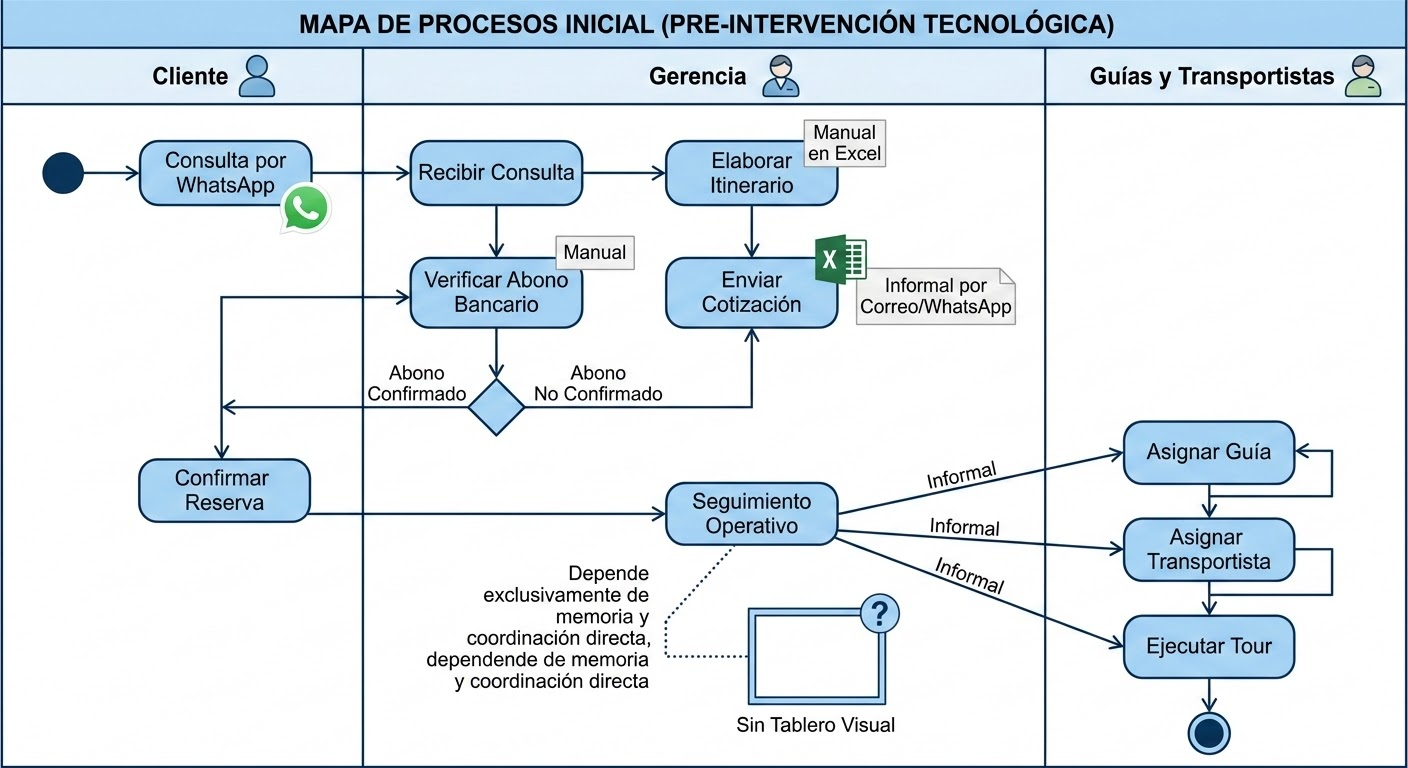
\includegraphics[width=\textwidth]{assets/mapa-procesos-inicial.jpg}
    \caption{Mapa de procesos inicial de Machu Picchu Exclusive Tours}
\end{figure}

